\section{DIL\_\-ID  Class Reference}
\label{classDIL__ID}\index{DIL_ID@{DIL\_\-ID}}
{\tt \#include $<$dil2al.hh$>$}

Inheritance diagram for DIL\_\-ID::\begin{figure}[H]
\begin{center}
\leavevmode
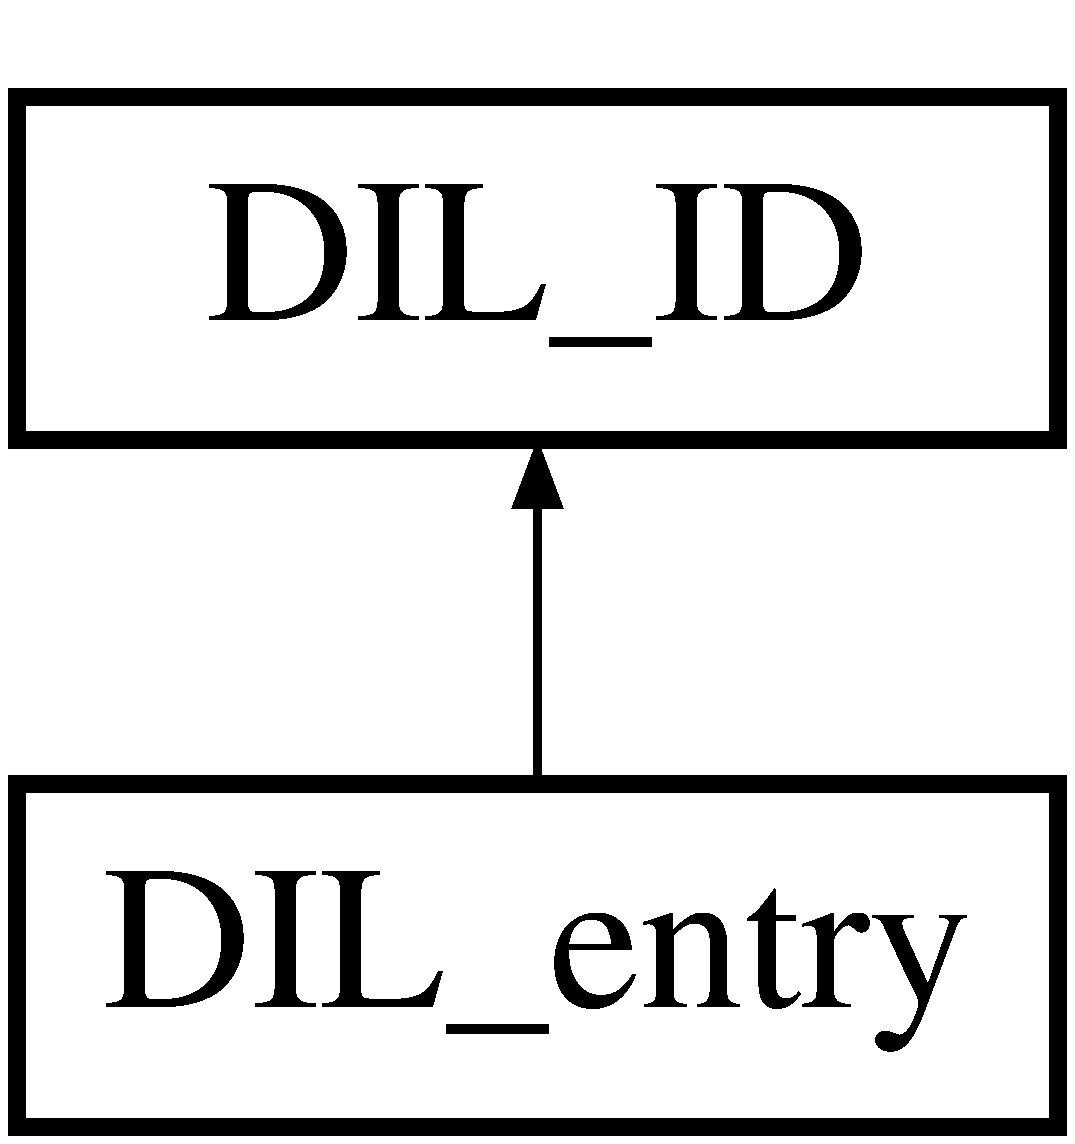
\includegraphics[height=2cm]{classDIL__ID}
\end{center}
\end{figure}
\subsection*{Public Methods}
\begin{CompactItemize}
\item 
{\bf DIL\_\-ID} ()
\item 
{\bf DIL\_\-ID} ({\bf idnumber} idmaj0, {\bf idnumber} idmaj1, unsigned int idmin)
\item 
{\bf DIL\_\-ID} (DIL\_\-ID \&id)
\item 
{\bf DIL\_\-ID} ({\bf String} \&idstr)
\item 
{\bf DIL\_\-ID} (const {\bf Sub\-String} \&idstr)
\item 
DIL\_\-ID \& {\bf operator=} (const DIL\_\-ID \&id)
\item 
bool {\bf operator==} (const DIL\_\-ID \&id2) const
\item 
bool {\bf operator!=} (const DIL\_\-ID \&id2) const
\item 
bool {\bf operator$<$} (const DIL\_\-ID \&id2) const
\item 
bool {\bf operator$<$=} (const DIL\_\-ID \&id2) const
\item 
bool {\bf operator$>$} (const DIL\_\-ID \&id2) const
\item 
bool {\bf operator$>$=} (const DIL\_\-ID \&id2) const
\item 
DIL\_\-ID \& {\bf operator=} ({\bf String} \&idstr)
\item 
DIL\_\-ID \& {\bf operator=} ({\bf String} $\ast$idstr)
\item 
{\bf String} {\bf str} () const
\item 
const char $\ast$ {\bf chars} () const
\item 
{\bf operator const char $\ast$} () const
\item 
bool {\bf valid} ()
\item 
bool {\bf Write\_\-DIL\_\-ID\_\-to\_\-Binary\_\-Cache} (ofstream \&cfl)
\item 
bool {\bf Read\_\-DIL\_\-ID\_\-from\_\-Binary\_\-Cache} (ifstream \&cfl)
\end{CompactItemize}
\subsection*{Public Attributes}
\begin{CompactItemize}
\item 
{\bf idnumber} {\bf idmajor} [2]
\item 
unsigned int {\bf idminor}
\end{CompactItemize}
\subsection*{Protected Methods}
\begin{CompactItemize}
\item 
void {\bf init} ({\bf String} \&idstr)
\end{CompactItemize}


\subsection{Constructor \& Destructor Documentation}
\index{DIL_ID@{DIL\_\-ID}!DIL_ID@{DIL\_\-ID}}
\index{DIL_ID@{DIL\_\-ID}!DIL_ID@{DIL\_\-ID}}
\subsubsection{\setlength{\rightskip}{0pt plus 5cm}DIL\_\-ID::DIL\_\-ID ()\hspace{0.3cm}{\tt  [inline]}}\label{classDIL__ID_a0}




Definition at line 410 of file dil2al.hh.

References idmajor, and idminor.



\footnotesize\begin{verbatim}410 : idminor(0) { idmajor[0]=0; idmajor[1]=0; }
\end{verbatim}\normalsize 
\index{DIL_ID@{DIL\_\-ID}!DIL_ID@{DIL\_\-ID}}
\index{DIL_ID@{DIL\_\-ID}!DIL_ID@{DIL\_\-ID}}
\subsubsection{\setlength{\rightskip}{0pt plus 5cm}DIL\_\-ID::DIL\_\-ID ({\bf idnumber} {\em idmaj0}, {\bf idnumber} {\em idmaj1}, unsigned int {\em idmin})\hspace{0.3cm}{\tt  [inline]}}\label{classDIL__ID_a1}




Definition at line 411 of file dil2al.hh.

References idmajor, idminor, and idnumber.



\footnotesize\begin{verbatim}411 : idminor(idmin) { idmajor[0]=idmaj0; idmajor[1]=idmaj1; }
\end{verbatim}\normalsize 
\index{DIL_ID@{DIL\_\-ID}!DIL_ID@{DIL\_\-ID}}
\index{DIL_ID@{DIL\_\-ID}!DIL_ID@{DIL\_\-ID}}
\subsubsection{\setlength{\rightskip}{0pt plus 5cm}DIL\_\-ID::DIL\_\-ID (DIL\_\-ID \& {\em id})\hspace{0.3cm}{\tt  [inline]}}\label{classDIL__ID_a2}




Definition at line 412 of file dil2al.hh.

References idmajor, and idminor.



\footnotesize\begin{verbatim}412 : idminor(id.idminor) { idmajor[0]=id.idmajor[0]; idmajor[1]=id.idmajor[1]; }
\end{verbatim}\normalsize 
\index{DIL_ID@{DIL\_\-ID}!DIL_ID@{DIL\_\-ID}}
\index{DIL_ID@{DIL\_\-ID}!DIL_ID@{DIL\_\-ID}}
\subsubsection{\setlength{\rightskip}{0pt plus 5cm}DIL\_\-ID::DIL\_\-ID ({\bf String} \& {\em idstr})\hspace{0.3cm}{\tt  [inline]}}\label{classDIL__ID_a3}




Definition at line 413 of file dil2al.hh.

References init().



\footnotesize\begin{verbatim}413 { init(idstr); }
\end{verbatim}\normalsize 
\index{DIL_ID@{DIL\_\-ID}!DIL_ID@{DIL\_\-ID}}
\index{DIL_ID@{DIL\_\-ID}!DIL_ID@{DIL\_\-ID}}
\subsubsection{\setlength{\rightskip}{0pt plus 5cm}DIL\_\-ID::DIL\_\-ID (const {\bf Sub\-String} \& {\em idstr})\hspace{0.3cm}{\tt  [inline]}}\label{classDIL__ID_a4}




Definition at line 414 of file dil2al.hh.

References init().



\footnotesize\begin{verbatim}414 { String s(idstr); init(s); }
\end{verbatim}\normalsize 


\subsection{Member Function Documentation}
\index{DIL_ID@{DIL\_\-ID}!chars@{chars}}
\index{chars@{chars}!DIL_ID@{DIL\_\-ID}}
\subsubsection{\setlength{\rightskip}{0pt plus 5cm}const char$\ast$ DIL\_\-ID::chars () const\hspace{0.3cm}{\tt  [inline]}}\label{classDIL__ID_a15}




Definition at line 444 of file dil2al.hh.

References String::chars(), and str().

Referenced by Active\_\-List::Active\_\-List(), DIL\_\-Required\_\-Task\_\-Chunks(), generate\_\-AL(), generate\_\-EPS\_\-cells(), Active\_\-List::generate\_\-focused\_\-AL(), generate\_\-modify\_\-element\_\-FORM\_\-interface\_\-DIL\_\-entry\_\-content(), generate\_\-modify\_\-element\_\-FORM\_\-interface\_\-DIL\_\-entry\_\-parameters(), Active\_\-List::generate\_\-wide\_\-AL(), Detailed\_\-Items\_\-List::Get\_\-All\_\-DIL\_\-ID\_\-File\_\-Parameters(), Detailed\_\-Items\_\-List::Get\_\-All\_\-Topical\_\-DIL\_\-Parameters(), modify\_\-DIL\_\-entry\_\-target\_\-date(), modify\_\-DIL\_\-group\_\-target\_\-dates(), modify\_\-DIL\_\-group\_\-target\_\-dates\_\-cmd(), modify\_\-element\_\-through\_\-FORM\_\-interface(), operator const char $\ast$(), DIL\_\-entry::Propagated\_\-Target\_\-Date(), Detailed\_\-Items\_\-List::Read\_\-Topical\_\-from\_\-Binary\_\-Cache(), Show\_\-DIL\_\-Hierarchy(), update\_\-DIL\_\-entry\_\-parameter\_\-elements(), update\_\-DIL\_\-to\_\-AL(), update\_\-main\_\-ALs(), DIL\_\-Visualize\_\-with\_\-FORM\_\-Tabs::Visualize\_\-Element(), DIL\_\-Visualize\_\-with\_\-HTML\_\-Tabs::Visualize\_\-Element(), and DIL\_\-Visualize\_\-with\_\-Tabs::Visualize\_\-Element().



\footnotesize\begin{verbatim}444                                    { 
445     /*cout << "CHECKING: ";
446       for (char * tp = (char *) str().chars(); *tp!='\0'; tp++) cout << (*tp) << '[' << (int) (*tp) << ']';
447       cout << '\n';*/
448     /*String idstr(str());
449       cout << "idstr in chars() function: ";
450       int i = 0;
451       for (char * tp = (char *) idstr.chars(); (*tp!='\0') && (i<80); tp++, i++) cout << (*tp) << '{' << (int) (*tp) << '}';
452       cout << '\n';*/
453     static String idstr; // need static here to avoid trouble with life-time of object that chars() return points to
454     idstr = str();
455     return idstr.chars(); }
\end{verbatim}\normalsize 
\index{DIL_ID@{DIL\_\-ID}!init@{init}}
\index{init@{init}!DIL_ID@{DIL\_\-ID}}
\subsubsection{\setlength{\rightskip}{0pt plus 5cm}void DIL\_\-ID::init ({\bf String} \& {\em idstr})\hspace{0.3cm}{\tt  [inline, protected]}}\label{classDIL__ID_b0}




Definition at line 401 of file dil2al.hh.

References String::after(), String::at(), String::before(), String::from(), idmajor, idminor, and String::length().

Referenced by DIL\_\-ID(), and operator=().



\footnotesize\begin{verbatim}401                             {
402     String idmajorstr(idstr.before('.'));
403     idmajor[0] = (idnumber) atol((const char *) String(idmajorstr.at(0,idmajorstr.length()-6)));
404     idmajor[1] = (idnumber) atol((const char *) String(idmajorstr.from(((int) idmajorstr.length())-6)));
405     idminor = (unsigned int) atoi((const char *) String(idstr.after('.')));
406   }
\end{verbatim}\normalsize 
\index{DIL_ID@{DIL\_\-ID}!operator const char *@{operator const char $\ast$}}
\index{operator const char *@{operator const char $\ast$}!DIL_ID@{DIL\_\-ID}}
\subsubsection{\setlength{\rightskip}{0pt plus 5cm}DIL\_\-ID::operator const char $\ast$ () const\hspace{0.3cm}{\tt  [inline]}}\label{classDIL__ID_a16}




Definition at line 456 of file dil2al.hh.

References chars().



\footnotesize\begin{verbatim}456 { return chars(); }
\end{verbatim}\normalsize 
\index{DIL_ID@{DIL\_\-ID}!operator"!=@{operator"!=}}
\index{operator"!=@{operator"!=}!DIL_ID@{DIL\_\-ID}}
\subsubsection{\setlength{\rightskip}{0pt plus 5cm}bool DIL\_\-ID::operator!= (const DIL\_\-ID \& {\em id2}) const\hspace{0.3cm}{\tt  [inline]}}\label{classDIL__ID_a7}




Definition at line 425 of file dil2al.hh.



\footnotesize\begin{verbatim}425 { return (!(*this==id2)); }
\end{verbatim}\normalsize 
\index{DIL_ID@{DIL\_\-ID}!operator<@{operator$<$}}
\index{operator<@{operator$<$}!DIL_ID@{DIL\_\-ID}}
\subsubsection{\setlength{\rightskip}{0pt plus 5cm}bool DIL\_\-ID::operator$<$ (const DIL\_\-ID \& {\em id2}) const\hspace{0.3cm}{\tt  [inline]}}\label{classDIL__ID_a8}




Definition at line 426 of file dil2al.hh.

References idmajor, and idminor.



\footnotesize\begin{verbatim}426 { return ((idmajor[0]<id2.idmajor[0]) || ((idmajor[0]==id2.idmajor[0]) && (idmajor[1]<id2.idmajor[1])) || ((idmajor[0]==id2.idmajor[0]) && (idmajor[1]==id2.idmajor[1]) && (idminor<id2.idminor))); }
\end{verbatim}\normalsize 
\index{DIL_ID@{DIL\_\-ID}!operator<=@{operator$<$=}}
\index{operator<=@{operator$<$=}!DIL_ID@{DIL\_\-ID}}
\subsubsection{\setlength{\rightskip}{0pt plus 5cm}bool DIL\_\-ID::operator$<$= (const DIL\_\-ID \& {\em id2}) const\hspace{0.3cm}{\tt  [inline]}}\label{classDIL__ID_a9}




Definition at line 427 of file dil2al.hh.



\footnotesize\begin{verbatim}427 { return ((*this<id2) || (*this==id2)); }
\end{verbatim}\normalsize 
\index{DIL_ID@{DIL\_\-ID}!operator=@{operator=}}
\index{operator=@{operator=}!DIL_ID@{DIL\_\-ID}}
\subsubsection{\setlength{\rightskip}{0pt plus 5cm}DIL\_\-ID\& DIL\_\-ID::operator= ({\bf String} $\ast$ {\em idstr})\hspace{0.3cm}{\tt  [inline]}}\label{classDIL__ID_a13}




Definition at line 432 of file dil2al.hh.

References init().



\footnotesize\begin{verbatim}432 { init(*idstr); }
\end{verbatim}\normalsize 
\index{DIL_ID@{DIL\_\-ID}!operator=@{operator=}}
\index{operator=@{operator=}!DIL_ID@{DIL\_\-ID}}
\subsubsection{\setlength{\rightskip}{0pt plus 5cm}DIL\_\-ID\& DIL\_\-ID::operator= ({\bf String} \& {\em idstr})\hspace{0.3cm}{\tt  [inline]}}\label{classDIL__ID_a12}




Definition at line 431 of file dil2al.hh.

References init().



\footnotesize\begin{verbatim}431 { init(idstr); }
\end{verbatim}\normalsize 
\index{DIL_ID@{DIL\_\-ID}!operator=@{operator=}}
\index{operator=@{operator=}!DIL_ID@{DIL\_\-ID}}
\subsubsection{\setlength{\rightskip}{0pt plus 5cm}DIL\_\-ID\& DIL\_\-ID::operator= (const DIL\_\-ID \& {\em id})\hspace{0.3cm}{\tt  [inline]}}\label{classDIL__ID_a5}




Definition at line 423 of file dil2al.hh.

References idmajor, and idminor.



\footnotesize\begin{verbatim}423 { idmajor[0]=id.idmajor[0]; idmajor[1]=id.idmajor[1]; idminor=id.idminor; return *this; }
\end{verbatim}\normalsize 
\index{DIL_ID@{DIL\_\-ID}!operator==@{operator==}}
\index{operator==@{operator==}!DIL_ID@{DIL\_\-ID}}
\subsubsection{\setlength{\rightskip}{0pt plus 5cm}bool DIL\_\-ID::operator== (const DIL\_\-ID \& {\em id2}) const\hspace{0.3cm}{\tt  [inline]}}\label{classDIL__ID_a6}




Definition at line 424 of file dil2al.hh.

References idmajor, and idminor.



\footnotesize\begin{verbatim}424 { return ((idmajor[0]==id2.idmajor[0]) && (idmajor[1]==id2.idmajor[1]) && (idminor==id2.idminor)); }
\end{verbatim}\normalsize 
\index{DIL_ID@{DIL\_\-ID}!operator>@{operator$>$}}
\index{operator>@{operator$>$}!DIL_ID@{DIL\_\-ID}}
\subsubsection{\setlength{\rightskip}{0pt plus 5cm}bool DIL\_\-ID::operator$>$ (const DIL\_\-ID \& {\em id2}) const\hspace{0.3cm}{\tt  [inline]}}\label{classDIL__ID_a10}




Definition at line 428 of file dil2al.hh.



\footnotesize\begin{verbatim}428 { return (id2<*this); }
\end{verbatim}\normalsize 
\index{DIL_ID@{DIL\_\-ID}!operator>=@{operator$>$=}}
\index{operator>=@{operator$>$=}!DIL_ID@{DIL\_\-ID}}
\subsubsection{\setlength{\rightskip}{0pt plus 5cm}bool DIL\_\-ID::operator$>$= (const DIL\_\-ID \& {\em id2}) const\hspace{0.3cm}{\tt  [inline]}}\label{classDIL__ID_a11}




Definition at line 429 of file dil2al.hh.



\footnotesize\begin{verbatim}429 { return (id2<=*this); }
\end{verbatim}\normalsize 
\index{DIL_ID@{DIL\_\-ID}!Read_DIL_ID_from_Binary_Cache@{Read\_\-DIL\_\-ID\_\-from\_\-Binary\_\-Cache}}
\index{Read_DIL_ID_from_Binary_Cache@{Read\_\-DIL\_\-ID\_\-from\_\-Binary\_\-Cache}!DIL_ID@{DIL\_\-ID}}
\subsubsection{\setlength{\rightskip}{0pt plus 5cm}bool DIL\_\-ID::Read\_\-DIL\_\-ID\_\-from\_\-Binary\_\-Cache (ifstream \& {\em cfl})}\label{classDIL__ID_a19}




Definition at line 542 of file utilities.cc.

References READSOMETYPE.

Referenced by DIL\_\-entry::Read\_\-from\_\-Binary\_\-Cache(), and Detailed\_\-Items\_\-List::Read\_\-Topical\_\-from\_\-Binary\_\-Cache().



\footnotesize\begin{verbatim}542                                                          {
543   // DIL_ID
544   if ((cfl.read((READSOMETYPE) this, sizeof(DIL_ID))).gcount()<sizeof(DIL_ID)) return false;
545   // alternative code:
546   //  if ((cfl.read((READSOMETYPE) idmajor, sizeof(idnumber)*2)).gcount()<(sizeof(idnumber)*2)) return false;
547   //  if ((cfl.read((READSOMETYPE) (&idminor), sizeof(idminor))).gcount()<sizeof(idminor)) return false;
548   return true;
549 }
\end{verbatim}\normalsize 
\index{DIL_ID@{DIL\_\-ID}!str@{str}}
\index{str@{str}!DIL_ID@{DIL\_\-ID}}
\subsubsection{\setlength{\rightskip}{0pt plus 5cm}{\bf String} DIL\_\-ID::str () const}\label{classDIL__ID_a14}




Definition at line 523 of file utilities.cc.

References idmajor, idminor, String::length(), and String::prepend().

Referenced by chars(), Active\_\-List::generate\_\-focused\_\-AL(), DIL\_\-AL\_\-List::Is\-Self\-Reference(), modify\_\-element\_\-through\_\-FORM\_\-interface(), DIL\_\-entry::Propagated\_\-Target\_\-Date(), Detailed\_\-Items\_\-List::Read\_\-from\_\-Binary\_\-Cache(), DIL\_\-Visualize\_\-with\_\-FORM\_\-Tabs::Visualize\_\-Element(), and DIL\_\-Visualize\_\-with\_\-FORM\_\-Tabs::Visualize\_\-Plan\_\-Entry().



\footnotesize\begin{verbatim}523                          {
524         static String idstr; // stored in function, not objects, static to avoid problems with lifetime of object that return value points to
525         idstr = String((long) idmajor[1]);
526         while (idstr.length()<6) idstr.prepend('0');
527         idstr.prepend(String((long) idmajor[0]));
528         idstr += '.' + String((long) idminor);
529 /*cout << "chars() RESULT at end of str() function: ";
530 int i = 0;
531 for (char * tp = (char *) idstr.chars(); (*tp!='\0') && (i<80); tp++, i++) cout << (*tp) << '{' << (int) (*tp) << '}';
532 cout << '\n';*/
533         return idstr;
534 }
\end{verbatim}\normalsize 
\index{DIL_ID@{DIL\_\-ID}!valid@{valid}}
\index{valid@{valid}!DIL_ID@{DIL\_\-ID}}
\subsubsection{\setlength{\rightskip}{0pt plus 5cm}bool DIL\_\-ID::valid ()\hspace{0.3cm}{\tt  [inline]}}\label{classDIL__ID_a17}




Definition at line 458 of file dil2al.hh.

References idmajor, and idminor.

Referenced by generate\_\-modify\_\-element\_\-FORM\_\-interface(), generate\_\-modify\_\-element\_\-FORM\_\-interface\_\-DIL\_\-entry\_\-parameters(), Detailed\_\-Items\_\-List::Get\_\-All\_\-DIL\_\-ID\_\-File\_\-Parameters(), DIL\_\-AL\_\-List::Is\-Self\-Reference(), modify\_\-element\_\-through\_\-FORM\_\-interface(), Plan\_\-entry\_\-content::Parse\_\-Entry\_\-Content(), DIL\_\-entry::Propagated\_\-Target\_\-Date(), DIL\_\-AL\_\-List::Superiorbyid(), Tabbed\_\-DIL\_\-Hierarchy(), Tabbed\_\-FORM\_\-DIL\_\-Hierarchy(), and Tabbed\_\-HTML\_\-DIL\_\-Hierarchy().



\footnotesize\begin{verbatim}458 { return ((idmajor[0]!=0) && (idmajor[1]!=0) && (idminor!=0)); }
\end{verbatim}\normalsize 
\index{DIL_ID@{DIL\_\-ID}!Write_DIL_ID_to_Binary_Cache@{Write\_\-DIL\_\-ID\_\-to\_\-Binary\_\-Cache}}
\index{Write_DIL_ID_to_Binary_Cache@{Write\_\-DIL\_\-ID\_\-to\_\-Binary\_\-Cache}!DIL_ID@{DIL\_\-ID}}
\subsubsection{\setlength{\rightskip}{0pt plus 5cm}bool DIL\_\-ID::Write\_\-DIL\_\-ID\_\-to\_\-Binary\_\-Cache (ofstream \& {\em cfl})}\label{classDIL__ID_a18}




Definition at line 536 of file utilities.cc.

Referenced by DIL\_\-entry::Write\_\-to\_\-Binary\_\-Cache(), and DIL\_\-entry::Write\_\-Topical\_\-to\_\-Binary\_\-Cache().



\footnotesize\begin{verbatim}536                                                         {
537   // DIL_ID
538   cfl.write((const void *) this, sizeof(DIL_ID));
539   return true;
540 }
\end{verbatim}\normalsize 


\subsection{Member Data Documentation}
\index{DIL_ID@{DIL\_\-ID}!idmajor@{idmajor}}
\index{idmajor@{idmajor}!DIL_ID@{DIL\_\-ID}}
\subsubsection{\setlength{\rightskip}{0pt plus 5cm}{\bf idnumber} DIL\_\-ID::idmajor[2]}\label{classDIL__ID_m0}




Definition at line 420 of file dil2al.hh.

Referenced by DIL\_\-ID(), init(), operator$<$(), operator=(), operator==(), str(), and valid().\index{DIL_ID@{DIL\_\-ID}!idminor@{idminor}}
\index{idminor@{idminor}!DIL_ID@{DIL\_\-ID}}
\subsubsection{\setlength{\rightskip}{0pt plus 5cm}unsigned int DIL\_\-ID::idminor}\label{classDIL__ID_m1}




Definition at line 421 of file dil2al.hh.

Referenced by DIL\_\-ID(), init(), operator$<$(), operator=(), operator==(), str(), and valid().

The documentation for this class was generated from the following files:\begin{CompactItemize}
\item 
{\bf dil2al.hh}\item 
{\bf utilities.cc}\end{CompactItemize}
